\documentclass[first=orange,second=blue,logo=blueque]{aaltoslides}

\usepackage[utf8]{inputenc}
\usepackage[T1]{fontenc}
\usepackage{graphicx}
\usepackage{amssymb,amsmath}
\usepackage{url}
\usepackage{lastpage}

\newcommand{\SubItem}[1]{
    {\setlength\itemindent{15pt} \item[$\bullet$] #1}
}

\title{Utilisation of viewing statistics in video recording credits detection}

\author[S. Kivistö]{Saskia Kivistö}
%\institute[ICS]{Department of Computer Science\\
%Aalto University, School of Science \\saskia.kivisto@aalto.fi}
\institute[ICS]{Bachelor's thesis presentation}

\aaltofootertext{Bachelor's thesis presentation}{April 14, 2022}{\insertframenumber/\inserttotalframenumber}

\date{April 14, 2022}

\begin{document}
%TODO: why user behaviour data?

%%%%%%%%%%%%%%%%%%%%%%%%%%%%%%%%%%%%%%%%%%%%%%%%%%%%%%%%%%%%%%%%%%%%%%%%%%%%%%%%%%%%%%%%%%%%%

\aaltotitleframe

%%%%%%%%%%%%%%%%%%%%%%%%%%%%%%%%%%%%%%%%%%%%%%%%%%%%%%%%%%%%%%%%%%%%%%%%%%%%%%%%%%%%%%%%%%%%%

\begin{frame}{1. Introduction}
    \begin{enumerate}
        \alert{\item Introduction}
        \item User viewing behaviour data
        \item Problem formulation and methods
        \item Results
    \end{enumerate}
\end{frame}

%%%%%%%%%%%%%%%%%%%%%%%%%%%%%%%%%%%%%%%%%%%%%%%%%%%%%%%%%%%%%%%%%%%%%%%%%%%%%%%%%%%%%%%%%%%%%

\begin{frame}{1. Introduction}
    \begin{block}{{\color{black}Goal of this thesis:}}
        \begin{itemize}
        \item Detect where recorded TV programs actually start and end
        \item by analysing patterns of user viewing behaviour
        \end{itemize}
    \end{block}
\end{frame}

%%%%%%%%%%%%%%%%%%%%%%%%%%%%%%%%%%%%%%%%%%%%%%%%%%%%%%%%%%%%%%%%%%%%%%%%%%%%%%%%%%%%%%%%%%%%%

\begin{frame}{1. Introduction}
    \begin{block}{{\color{black}The issue with recording TV programs:}}
        \begin{itemize}
            \item TV programs are not usually broadcasted exactly according to electronic program guide (EPG)
            \item Timing recording by EPG can lead to program being recorded only partially
            \item Buffer can be added to ensure that whole program is recorded
            \item Example recording of 10 o'clock news:
        \end{itemize}
        \center
        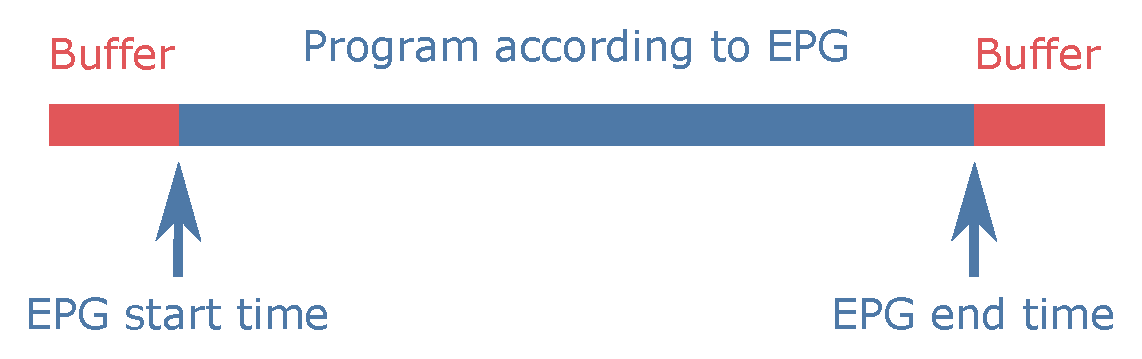
\includegraphics[width=1\textwidth]{figures/recording0.pdf}
    \end{block}
\end{frame}
    
%%%%%%%%%%%%%%%%%%%%%%%%%%%%%%%%%%%%%%%%%%%%%%%%%%%%%%%%%%%%%%%%%%%%%%%%%%%%%%%%%%%%%%%%%%%%%

\begin{frame}{1. Introduction}
    \begin{block}{{\color{black}The issue with recording TV programs:}}
        \begin{itemize}
            \item TV programs are not usually broadcasted exactly according to electronic program guide (EPG)
            \item Timing recording by EPG can lead to program being recorded only partially
            \item Buffer can be added to ensure that whole program is recorded
            \item Example recording of 10 o'clock news:
        \end{itemize}
        \center
        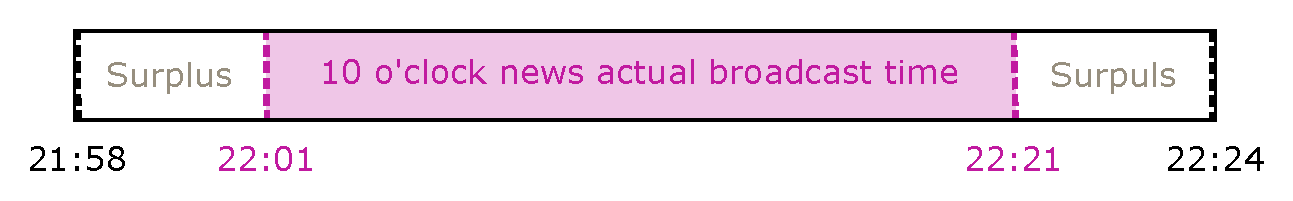
\includegraphics[width=1\textwidth]{figures/recording1.pdf}
    \end{block}
\end{frame}
    
%%%%%%%%%%%%%%%%%%%%%%%%%%%%%%%%%%%%%%%%%%%%%%%%%%%%%%%%%%%%%%%%%%%%%%%%%%%%%%%%%%%%%%%%%%%%%

\begin{frame}{1. Introduction}
    \begin{block}{{\color{black}}}
        \begin{itemize}
            \item Goal: identify surplus content
            \item Why?
                \SubItem{Its annoying to fast forward over surplus content}
                \SubItem{Surplus content consumes storage space}
        \end{itemize}
    \end{block}
\end{frame}
        
%%%%%%%%%%%%%%%%%%%%%%%%%%%%%%%%%%%%%%%%%%%%%%%%%%%%%%%%%%%%%%%%%%%%%%%%%%%%%%%%%%%%%%%%%%%%%

\begin{frame}{2. User viewing behaviour data}
    \begin{enumerate}
        \item Introduction
        \alert{\item User viewing behaviour data}
        \item Problem formulation and methods
        \item Results
    \end{enumerate}
\end{frame}

%%%%%%%%%%%%%%%%%%%%%%%%%%%%%%%%%%%%%%%%%%%%%%%%%%%%%%%%%%%%%%%%%%%%%%%%%%%%%%%%%%%%%%%%%%%%%

\begin{frame}{2. User viewing behaviour data}
    \begin{block}{{\color{black}\alert{Where} does the user behaviour data come from?}}
        \begin{itemize}
            \item The NPVR service provider company I am working for
            \item NPVR $\approx$ a normal video recorder
                \SubItem{but the TV programs you record are stored in a cloud server instead of a device in your home}
        \end{itemize}
    \end{block}
\end{frame}

%%%%%%%%%%%%%%%%%%%%%%%%%%%%%%%%%%%%%%%%%%%%%%%%%%%%%%%%%%%%%%%%%%%%%%%%%%%%%%%%%%%%%%%%%%%%%

\begin{frame}{2. User viewing behaviour data}
    \begin{block}{{\color{black}\alert{Why} is the data collected?}}
        \begin{itemize}
            %\item monitoring the popularity of programs
            \item To monitor the user experience quality
                \SubItem{smoothness of streaming etc.}
                \SubItem{with data related to the above, 
                it can be calculated \color{orange}{which parts of a recording were watched during a view, and which parts were fast forwarded}}
        \end{itemize}
    \end{block}
\end{frame}

%%%%%%%%%%%%%%%%%%%%%%%%%%%%%%%%%%%%%%%%%%%%%%%%%%%%%%%%%%%%%%%%%%%%%%%%%%%%%%%%%%%%%%%%%%%%%

\begin{frame}{2. User viewing behaviour data}
    \begin{block}{{\color{black}\alert{What} the examined data actually is?}}
        \begin{itemize}
            \item For each view of any recording, it can be calculated
                \\ {\color{orange}{which parts of the recording were watched during a view, and which parts were fast forwarded}}
            \item Users who record the same program will receive an identical recording
            \item \alert{User viewing behaviour data}:
            sum of viewed parts for recordings of the same program
            %aggregations of the views of a same program 
        \end{itemize}
    \end{block}
\end{frame}

%%%%%%%%%%%%%%%%%%%%%%%%%%%%%%%%%%%%%%%%%%%%%%%%%%%%%%%%%%%%%%%%%%%%%%%%%%%%%%%%%%%%%%%%%%%%%

\begin{frame}{2. User viewing behaviour data}
    \begin{block}{{\color{black}An example of the data}}
        \center
        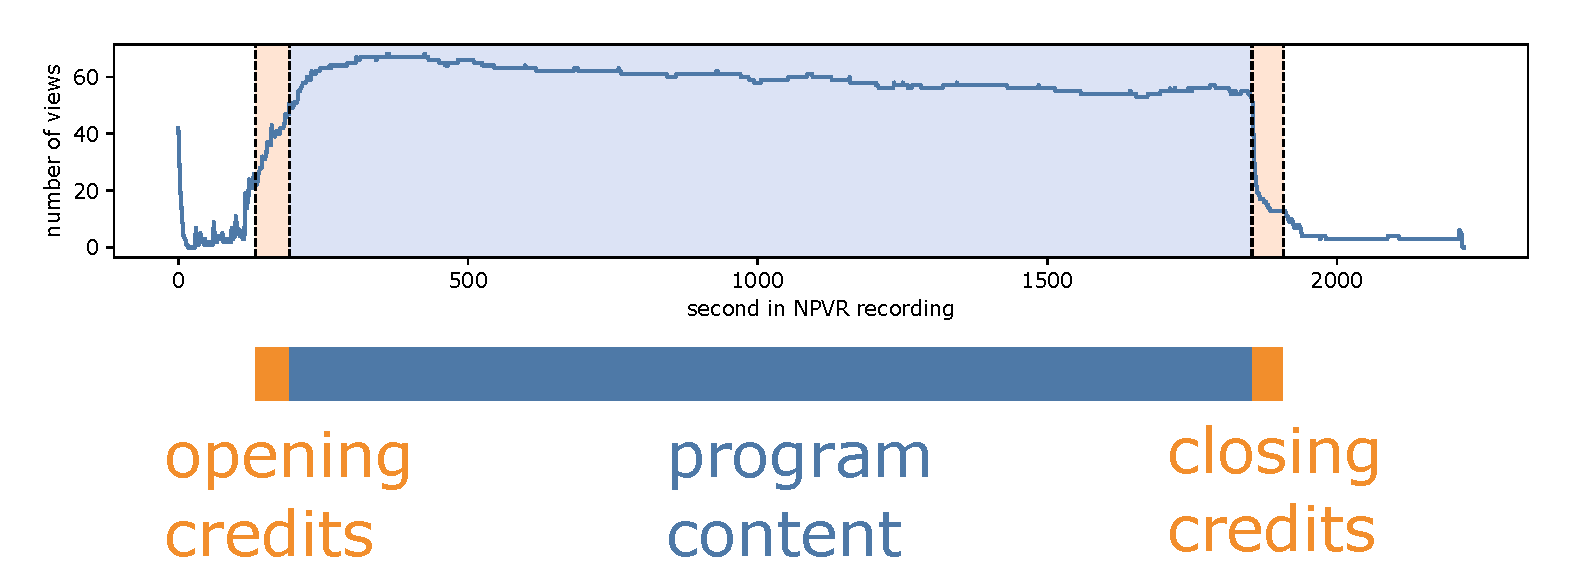
\includegraphics[width=1\textwidth]{figures/data1.pdf}
        \begin{itemize}
            \item Could credits be detected solely with this data?
        \end{itemize}
    \end{block}
\end{frame}

%%%%%%%%%%%%%%%%%%%%%%%%%%%%%%%%%%%%%%%%%%%%%%%%%%%%%%%%%%%%%%%%%%%%%%%%%%%%%%%%%%%%%%%%%%%%%

\begin{frame}{3. Problem formulation and methods}
    \begin{enumerate}
        \item Introduction
        \item User viewing behaviour data
        \alert{\item Problem formulation and methods}
        \item Results
    \end{enumerate}
\end{frame}

%%%%%%%%%%%%%%%%%%%%%%%%%%%%%%%%%%%%%%%%%%%%%%%%%%%%%%%%%%%%%%%%%%%%%%%%%%%%%%%%%%%%%%%%%%%%%

\begin{frame}{3. Problem formulation and methods}
    \begin{block}{{\color{black}An example of the data}}
        \center
        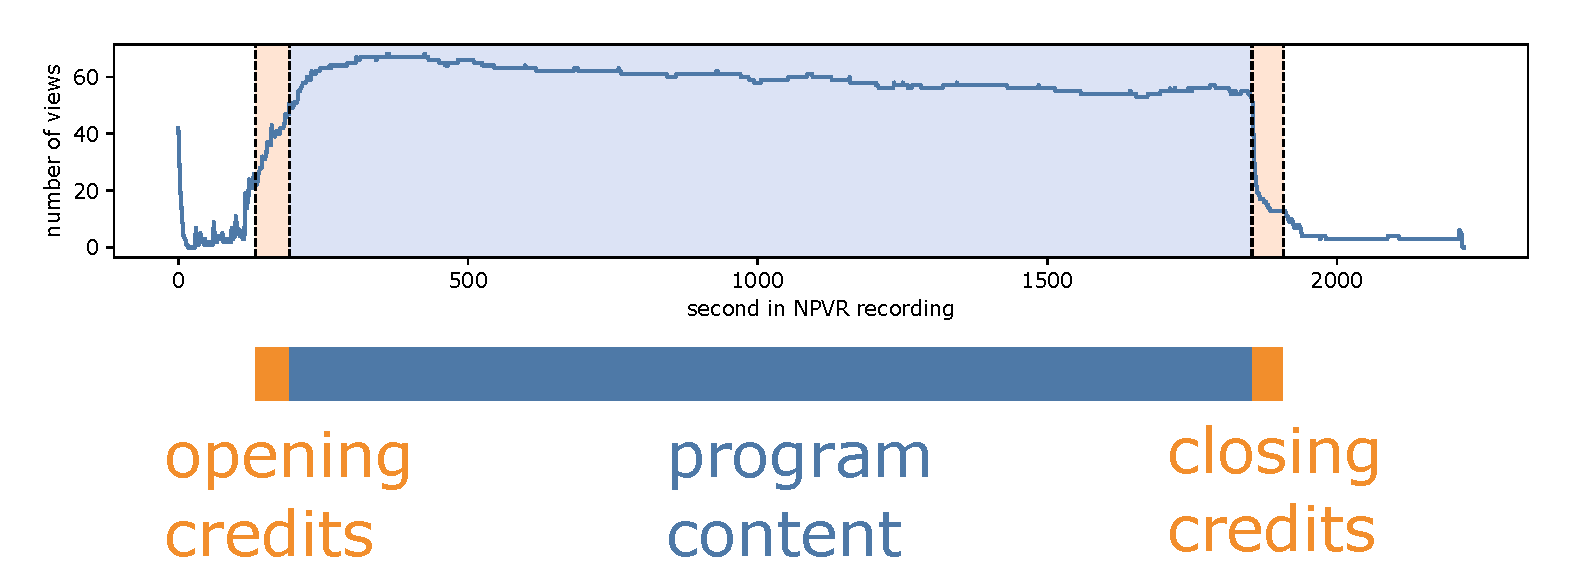
\includegraphics[width=1\textwidth]{figures/data1.pdf}
        \begin{itemize}
            \item Goal: try to find approximate location of credits
        \end{itemize}
    \end{block}
\end{frame}

%%%%%%%%%%%%%%%%%%%%%%%%%%%%%%%%%%%%%%%%%%%%%%%%%%%%%%%%%%%%%%%%%%%%%%%%%%%%%%%%%%%%%%%%%%%%%

\begin{frame}{3. Problem formulation and methods}
    \begin{block}{{\color{black}Problem formulation}}
        \begin{itemize}
            \item Signal processing, offline change point detection %(segmentation)
            \item Minimisation problem for the sum of costs of each segment (segments are divided by change points)
                \SubItem{cost function}
                \SubItem{search method}
            \item Python scientific library \texttt{ruptures} implements the above [1]
        \end{itemize}
    \end{block}
\end{frame}

%%%%%%%%%%%%%%%%%%%%%%%%%%%%%%%%%%%%%%%%%%%%%%%%%%%%%%%%%%%%%%%%%%%%%%%%%%%%%%%%%%%%%%%%%%%%%

\begin{frame}{3. Problem formulation and methods}
    \begin{block}{ {\color{black}Cost function} {\color{white}-----------------------------} {\color{white}Search method}}
        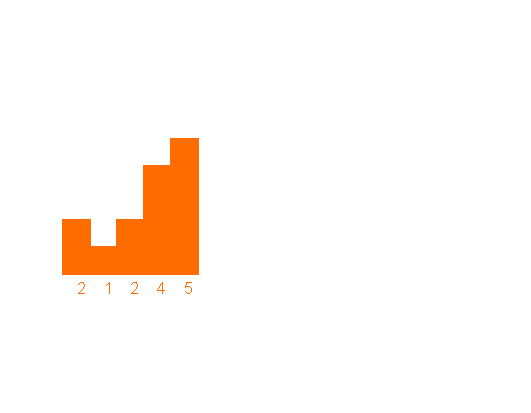
\includegraphics[width=0.49\textwidth]{figures/costfunction.pdf}
        
\includegraphics[width=0.49\textwidth]{figures/searchmethod_invisible.pdf}\\
        \vspace{-1cm} \hspace{0.5cm}
        \color{orange}{$\sigma^2=2,7$}
        \begin{itemize}
            \item \alert{cost function}: variance, detects distribution mean shifts well
        \end{itemize}
    \end{block}
\end{frame}

%%%%%%%%%%%%%%%%%%%%%%%%%%%%%%%%%%%%%%%%%%%%%%%%%%%%%%%%%%%%%%%%%%%%%%%%%%%%%%%%%%%%%%%%%%%%%

\begin{frame}{3. Problem formulation and methods}
    \begin{block}{ {\color{black}Cost function} {\color{white}-----------------------------} {\color{black}Search method}}
        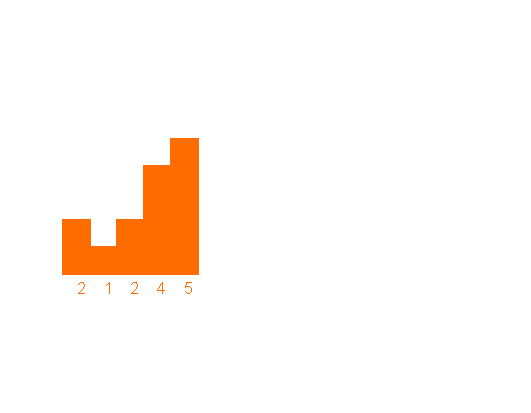
\includegraphics[width=0.49\textwidth]{figures/costfunction.pdf}
        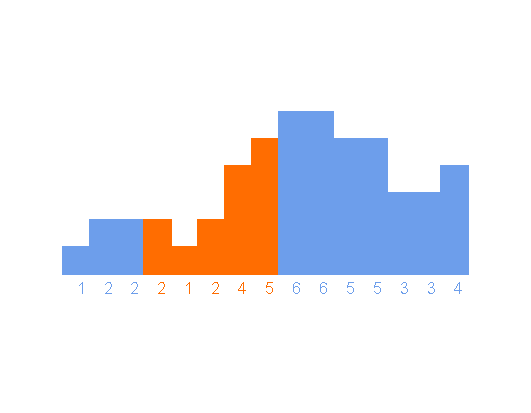
\includegraphics[width=0.49\textwidth]{figures/searchmethod.pdf}\\
        \vspace{-1cm} \hspace{0.5cm}
        \color{orange}{$\sigma^2=2,7$}
        \begin{itemize}
            \item \alert{cost function}: variance, detects distribution mean shifts well
            \item \alert{search method}: dynamic programming, produces optimal segmentation
        \end{itemize}
    \end{block}
\end{frame}

%%%%%%%%%%%%%%%%%%%%%%%%%%%%%%%%%%%%%%%%%%%%%%%%%%%%%%%%%%%%%%%%%%%%%%%%%%%%%%%%%%%%%%%%%%%%%

\begin{frame}{4. Results}
    \begin{enumerate}
        \item Introduction
        \item User viewing behaviour data
        \item Problem formulation and methods
        \alert{\item Results}
    \end{enumerate}
\end{frame}

%%%%%%%%%%%%%%%%%%%%%%%%%%%%%%%%%%%%%%%%%%%%%%%%%%%%%%%%%%%%%%%%%%%%%%%%%%%%%%%%%%%%%%%%%%%%%

\begin{frame}{4. Results}
    \begin{block}{{\color{black}Typical output}}
        \center
        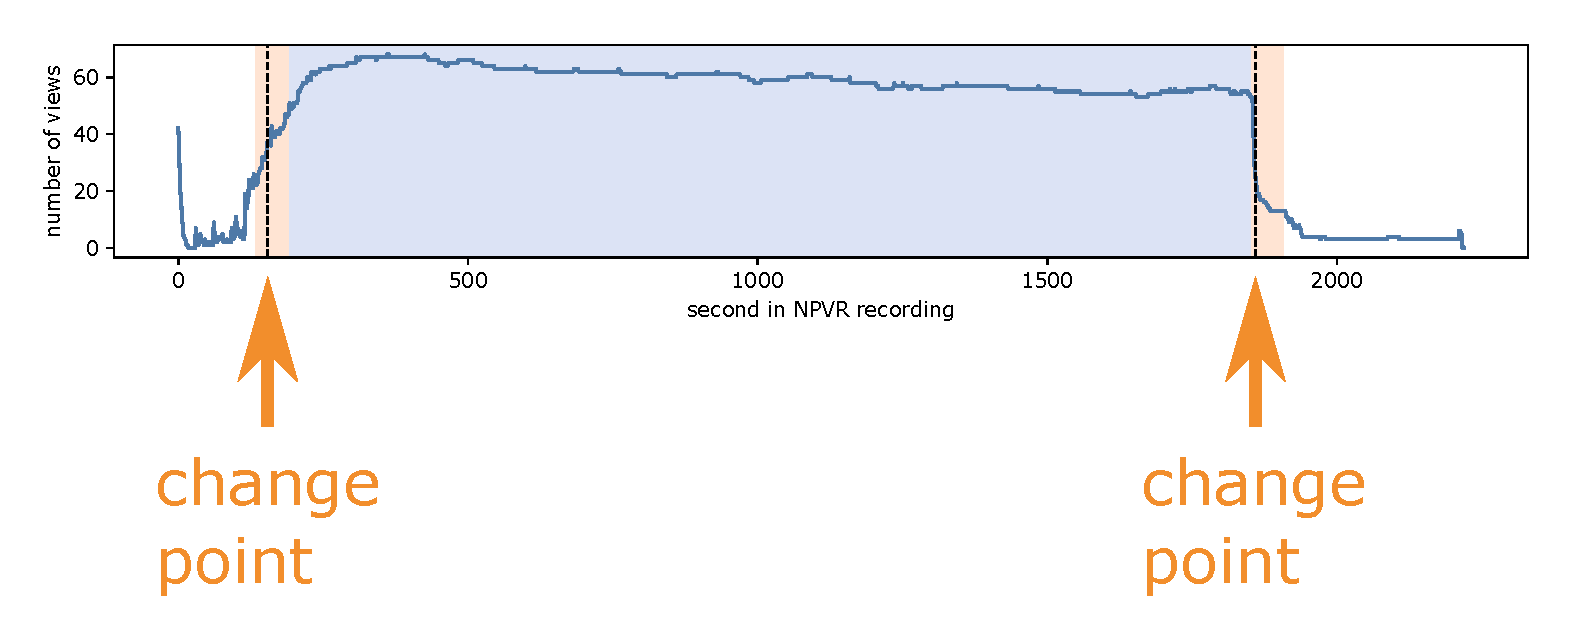
\includegraphics[width=1\textwidth]{figures/output1.pdf}
    \end{block}
\end{frame}

%%%%%%%%%%%%%%%%%%%%%%%%%%%%%%%%%%%%%%%%%%%%%%%%%%%%%%%%%%%%%%%%%%%%%%%%%%%%%%%%%%%%%%%%%%%%%

\begin{frame}{4. Results}
    \begin{block}{{\color{black}Predicted change point distance from closing credits start}}
        \center
        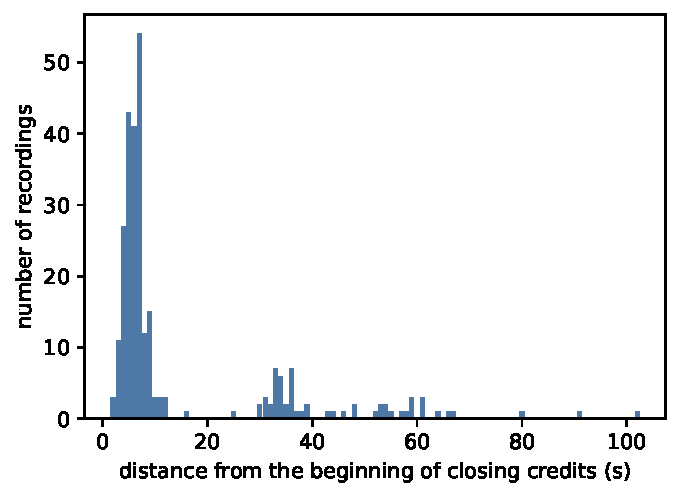
\includegraphics[width=0.7\textwidth]{figures/result_absolute0.pdf}
    \end{block}
\end{frame}

%%%%%%%%%%%%%%%%%%%%%%%%%%%%%%%%%%%%%%%%%%%%%%%%%%%%%%%%%%%%%%%%%%%%%%%%%%%%%%%%%%%%%%%%%%%%%

\begin{frame}{4. Results}
    \begin{block}{{\color{black}Can credits be detected based solely on user viewing behaviour?}}
        \begin{itemize}
            \item {\color{aaltoorange}{Yes}}, for approximate location of credits
            \item {\color{aaltoorange}{No}}, for exact start or end of credits
        \end{itemize}
    \end{block}
\end{frame}

%%%%%%%%%%%%%%%%%%%%%%%%%%%%%%%%%%%%%%%%%%%%%%%%%%%%%%%%%%%%%%%%%%%%%%%%%%%%%%%%%%%%%%%%%%%%%

\begin{frame}{Thank you!}
    %\center
    %\bfseries \Huge \color{aaltoorange} Thank you!
    \begin{block}{References}
        [1] Truong, C. \& Oudre, L. \& Vayatis, N. Selective review of offline change point detection methods. Signal Processing. 2020, vol. 167. P. 107299. Available at: doi:10.1016/j.sigpro.2019.107299.
    \end{block}
\end{frame}

\end{document}
